\begin{frame}{Probability}
    When we talked about the small sample malaria experiment, what we really wanted to know was, if the independence model is correct, what is the \textit{probability} that we'd see a difference as large as 64.3\%?
    \begin{itemize}
        \item Probability forms the foundation of statistics.
        \item You already know about a lot of these ideas!
        \begin{itemize}
            \item You may not have thought about them much, but you deal with probability automatically all the time. 
        \end{itemize}
        \item We are going to formalize these concepts.
    \end{itemize}
\end{frame}

\begin{frame}{Example: Rolling a Die}
    If you play any kind of dice-based tabletop games, you are probably familiar with weighing your options before making your next roll. This the kind of probability concept we want to formalize!
    
    \vspace{12pt}Suppose we have a six-sided die (d6). If we roll our d6 one time, what are the chances that we roll a \texttt{1}?
\end{frame}

\begin{frame}{Example: Rolling a Die}
    \begin{itemize}
        \item We assume that our d6 is a fair die, so it's not weighted toward any number in particular. 
        \item This means that all 6 numbers are equally likely.
        \item Therefore there is a 1-out-of-6 chance that we roll that \texttt{1}.
        \item When talking about probability, we write 1-out-of-6 as a fraction or decimal: $1/6 = 0.167$.
        \item We might also say that we have a 16.7\% chance of rolling a \texttt{1}.
    \end{itemize}
\end{frame}

\begin{frame}{Example 2: Rolling a Die}
    Suppose we need to roll at least a \texttt{4} to succeed in some game move. What are the chances that we succeed?
\end{frame}

\begin{frame}{Example 2: Rolling a Die}
    Suppose we need to roll at least a \texttt{4} to succeed in some game move. What are the chances that we succeed?
    \begin{itemize}
        \item To succeed, we can roll a \texttt{4}, \texttt{5}, or \texttt{6}.
        \item Our d6 has 6 sides and there are 3 numbers that result in success.
        \item Thus there is a 3-out-of-6 chance that we succeed, or $3/6 = 1/2 = 0.5$, a 50\% chance.
    \end{itemize}
\end{frame}

\begin{frame}{Example 3: Rolling a Die}
    What if we are interested in rolling a \texttt{1}, \texttt{2}, \texttt{3}, \texttt{4}, \texttt{5}, or \texttt{6}?
\end{frame}

\begin{frame}{Example 3: Rolling a Die}
    What if we are interested in rolling a \texttt{1}, \texttt{2}, \texttt{3}, \texttt{4}, \texttt{5}, or \texttt{6}?
    \begin{itemize}
        \item This is all of the possible sides.
        \item We have to roll at least one of those numbers (we cannot fail to roll a \texttt{1}, \texttt{2}, \texttt{3}, \texttt{4}, \texttt{5}, \textit{or} \texttt{6}).
        \item There is a 6-out-of-6 chance that we roll one of these numbers, or $6/6=1$ a 100\% chance.
    \end{itemize}
\end{frame}

\begin{frame}{Example 4: Rolling a Die}
    What if we are happy as long as we do \textbf{not} roll a \texttt{1}?
\end{frame}

\begin{frame}{Example 4: Rolling a Die}
    What if we are happy as long as we do \textbf{not} roll a 1?
    \begin{itemize}
        \item The chances of rolling a \texttt{1}, \texttt{2}, \texttt{3}, \texttt{4}, \texttt{5}, or \texttt{6} are 100\%.
        \item The chances of rolling a \texttt{1} are 16.7\%.
        \item So the chances of rolling a \texttt{2}, \texttt{3}, \texttt{4}, \texttt{5} , or \texttt{6} (but not a \texttt{1}) are $100\% - 16.7\% = 83.3\%$
    \end{itemize}
\end{frame}

\begin{frame}{Example 4: Rolling a Die}
    What if we are happy as long as we do \textbf{not} roll a \texttt{1}?
    \begin{itemize}
        \item Alternately, we can calculate this directly: not rolling a \texttt{1} means rolling a \texttt{2}, \texttt{3}, \texttt{4}, \texttt{5}, or \texttt{6}.
        \item The chances of rolling a \texttt{2}, \texttt{3}, \texttt{4}, \texttt{5}, or \texttt{6} are 5-out-of-6, or $5/6=0.833$, 83.3\%.
    \end{itemize}
\end{frame}

\begin{frame}{Example 5: Rolling a Die}
    What if we have 2d6? What is the chance that we roll two \texttt{1}s?
\end{frame}

\begin{frame}{Example 5: Rolling a Die}
    What if we have 2d6? What is the chance that we roll two \texttt{1}s?
    \begin{itemize}
        \item We know that there is a 1/6 chance that the first die is a \texttt{1}.
        \item Then, \textit{of those 1/6 times}, there is a 1/6 chance that the second die is a \texttt{1}.
        \item Then the chance that both dice roll a \texttt{1} is $(1/6)\times(1/6)=1/36$ or 2.78\%.
    \end{itemize}
\end{frame}

\begin{frame}{Example 5: Rolling a Die}
    We can also picture this in a table:
    \begin{table}[]
    \begin{tabular}{rccccccc}
    \multicolumn{1}{c}{}                                  &                        & \multicolumn{6}{c}{\texttt{first die}}                                                                                       \\
    \multicolumn{1}{c}{}                                  &                        & 1                     & 2                     & 3                     & 4                     & 5                     & 6                     \\ \cline{3-8} 
    \multirow{6}{*}{\texttt{second die}} & \multicolumn{1}{c|}{1} & \multicolumn{1}{c|}{\texttt{X}} & \multicolumn{1}{c|}{} & \multicolumn{1}{c|}{} & \multicolumn{1}{c|}{} & \multicolumn{1}{c|}{} & \multicolumn{1}{c|}{} \\ \cline{3-8} 
                                                      & \multicolumn{1}{c|}{2} & \multicolumn{1}{c|}{} & \multicolumn{1}{c|}{} & \multicolumn{1}{c|}{} & \multicolumn{1}{c|}{} & \multicolumn{1}{c|}{} & \multicolumn{1}{c|}{} \\ \cline{3-8} 
                                                      & \multicolumn{1}{c|}{3} & \multicolumn{1}{c|}{} & \multicolumn{1}{c|}{} & \multicolumn{1}{c|}{} & \multicolumn{1}{c|}{} & \multicolumn{1}{c|}{} & \multicolumn{1}{c|}{} \\ \cline{3-8} 
                                                      & \multicolumn{1}{c|}{4} & \multicolumn{1}{c|}{} & \multicolumn{1}{c|}{} & \multicolumn{1}{c|}{} & \multicolumn{1}{c|}{} & \multicolumn{1}{c|}{} & \multicolumn{1}{c|}{} \\ \cline{3-8} 
                                                      & \multicolumn{1}{c|}{5} & \multicolumn{1}{c|}{} & \multicolumn{1}{c|}{} & \multicolumn{1}{c|}{} & \multicolumn{1}{c|}{} & \multicolumn{1}{c|}{} & \multicolumn{1}{c|}{} \\ \cline{3-8} 
                                                      & \multicolumn{1}{c|}{6} & \multicolumn{1}{c|}{} & \multicolumn{1}{c|}{} & \multicolumn{1}{c|}{} & \multicolumn{1}{c|}{} & \multicolumn{1}{c|}{} & \multicolumn{1}{c|}{} \\ \cline{3-8} 
    \end{tabular}
    \end{table}
    There are 36 possible combinations (6 sides on the first die $\times$ 6 sides on the second die) and only one of them results in two ones: 1/36. 
\end{frame}

\begin{frame}{Probability}
    Whenever we mentioned the chance of something happening, we were also talking about the \textbf{probability} of something happening.
    \begin{itemize}
        \item We use probability to describe and understand \textbf{random processes} and their \textbf{outcomes}.
        \item In the previous examples, the random process is \textit{rolling a die} and the outcome is \textit{the number rolled}.
    \end{itemize}
\end{frame}

\begin{frame}{Probability}
    The \textbf{probability} of an outcome is the proportion of times the outcome would occur if we were able to observe the random process an infinite number of times.
\end{frame}

\begin{frame}{Probability}
    \begin{itemize}
        \item Probability is defined as a proportion and it \textit{always takes values between 0 and 1}.
        \begin{itemize}
            \item If you ever calculate a probability and get a number outside of 0 and 1, recalculate!
        \end{itemize}
        \item As a percentage, it takes values between 0\% and 100\%.
        \item A probability of 0 (0\%) means the outcome is impossible. 
        \item A probability of 1 (100\%) means that the outcome has to happen (all other outcomes are impossible).
    \end{itemize}
\end{frame}

\begin{frame}{Law of Large Numbers}
    We can illustrate probability by thinking about rolling a d6 and estimating the probability that we roll a \texttt{1}.
    \begin{itemize}
        \item We estimate this probability by counting up the number of times we roll a \texttt{1} and dividing by the number of times we rolled the d6.
        \item Each time we roll, we recalculate and our estimate will change a little bit.
        \item We denote this estimate $\hat{p}_n$, where $n$ is the number of rolls.
        \item We denote the true probability of rolling a \texttt{1} as $p=1/6$.
    \end{itemize}
\end{frame}

\begin{frame}{Law of Large Numbers}
    \begin{itemize}
        \item As the number of rolls, $n$, increases, $\hat{p}_n$ will get closer and closer to the true value of 1/6, or 16.7\%.
        \item We say that $\hat{p}_n$ \textit{converges} to the true probability.
        \item The tendency for $\hat{p}_n$ to converge to the true value as $n$ gets large is called the \textbf{Law of Large Numbers}. 
        \begin{itemize}
            \item This is another case of more data = better information!
        \end{itemize}
    \end{itemize}
\end{frame}

\begin{frame}{Law of Large Numbers}
    \begin{center}
        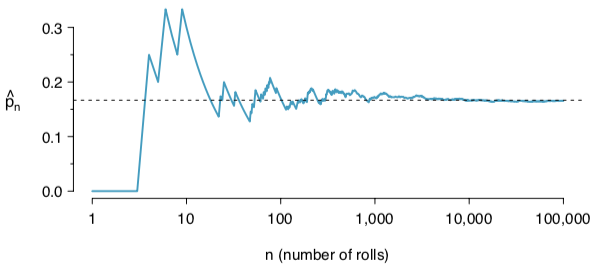
\includegraphics[scale=0.5]{images/lln.png}
    \end{center}
    With real-world data, we usually don't get a chance to see what happens when $n$ gets really big... but with simulations, we can see the Law of Large Numbers in action.
\end{frame}

\begin{frame}{Probability Notation}
    We have some shorthand notation for talking about probabilities.
    \begin{itemize}
        \item We denote "the probability of rolling a \texttt{1}" as P(rolling a \texttt{1}).
        \item As we get more comfortable with our notation, (assuming it's clear that we're talking about rolling a die) we may shorten this further to P(1).
        \item So we can write 
        \[P(\text{rolling a \texttt{1}}) = P(1) = 1/6.\]
    \end{itemize}
\end{frame}

\begin{frame}{Random Processes}
    Can you think of any other random processes we might want to examine? What are the possible outcomes?
\end{frame}

\begin{frame}{Random Processes}
    Here are a few random processes:
    \begin{itemize}
        \item Flipping a coin
        \item Wait time (in minutes) at the DMV
        \item How many hours of sleep you get each night
    \end{itemize}
    Some of these aren't completely random (the DMV is probably less crowded on, say, Tuesday mornings), but we may still want to model them based on random processes.
\end{frame}

\begin{frame}{Disjoint Outcomes}
    Two outcomes are \textbf{disjoint} or \textbf{mutually exclusive} if they cannot both happen.
    \begin{itemize}
        \item If we roll our d6 only one time, we cannot roll a \texttt{1} and a \texttt{2}. 
        \begin{itemize}
            \item On any single roll, the outcomes "rolling a \texttt{1}" and "rolling a \texttt{2}" are disjoint.
        \end{itemize}
        \item If one of a set of disjoint outcomes happens, it is impossible that any of the others can also happen.
    \end{itemize}
\end{frame}

\begin{frame}{Disjoint outcomes}
    It's easy to calculate probabilities for disjoint outcomes.
    
    \vspace{12pt}
    \begin{itemize}
        \item $P(\text{rolling a \texttt{1} \textbf{and} rolling a \texttt{2}}) = P(\text{\texttt{1} and \texttt{2}}) = 0$
        \begin{itemize}
            \item We can roll either a \texttt{1} or a \texttt{2}, but not both (on the same roll).
        \end{itemize}
        \item $P(\text{\texttt{1} \textbf{or} \texttt{2}}) = P(\text{\texttt{1}}) + P(\text{\texttt{2}}) = 1/6 + 1/6 = 1/3$
        \begin{itemize}
            \item If we want to roll a \texttt{1} or \texttt{2}, we have a 2-out-of-6 or $2/6=1/3$ chance.
        \end{itemize}
    \end{itemize}
\end{frame}

\begin{frame}{Addition Rule for Disjoint outcomes}
    We can formalize this relationship with the \textbf{addition rule for disjoint outcomes}. Suppose $A_1$ and $A_2$ are two disjoint outcomes. Then
    \[
        P(A_1 \text{ or } A_2) = P(A_1)+P(A_2).
    \]
    This can be extended to many disjoint outcomes $A_1, \dots, A_k$ where the probability that at least one of these outcomes will occur is
    \[
        P(A_1)+P(A_2)+\dots+P(A_k).
    \]
\end{frame}

\begin{frame}{Example}
    Recall our contingency table for \texttt{homeownership} and \texttt{apptype}: 
    \begin{center}
        \begin{tabular}{r l ccc r}
		& & \multicolumn{3}{c}{{\texttt{homeownership}}} & \\
        \cline{3-5}
		& & Rent & Mortgage & Own & Total  \\ 
        \cline{2-6}
        \multirow{2}{*}{{\texttt{apptype}}} 
        & Individual & 3496 & 3839 & 1170 & 8505 \\ 
  		& Joint & 362 & 950 & 183 & 1495 \\ 
        \cline{2-6}
  		& Total	& 3858 & 4789 & 1353 & 10000 \\
        \cline{2-6}
    \end{tabular}
    \end{center}
    \begin{enumerate}
        \item Are the outcomes Rent, Mortgage, and Own disjoint? Are Rent and Individual disjoint?
        \item What is the probability that someone applied for a joint loan? That someone is a renter and applied for an individual loan?
        \item Compute the probability that someone has a mortgage or owns their home.
    \end{enumerate}
\end{frame}

\begin{frame}{Example}
    \textbf{Are the outcomes Rent, Mortgage, and Own disjoint? Are Rent and Individual disjoint?}
    \begin{center}
        \begin{tabular}{r l ccc r}
		& & \multicolumn{3}{c}{{\texttt{homeownership}}} & \\
        \cline{3-5}
		& & Rent & Mortgage & Own & Total  \\ 
        \cline{2-6}
        \multirow{2}{*}{{\texttt{apptype}}} 
        & Individual & 3496 & 3839 & 1170 & 8505 \\ 
  		& Joint & 362 & 950 & 183 & 1495 \\ 
        \cline{2-6}
  		& Total	& 3858 & 4789 & 1353 & 10000 \\
        \cline{2-6}
    \end{tabular}
    \end{center}
    \vspace{12pt}Rent, Mortgage, and Own are disjoint outcomes. Someone either rents \textit{or} has a mortgage \textit{or} owns their home outright.
    
    \vspace{12pt}Rent and Individual are \textit{not} disjoint outcomes. It is possible to be a renter and apply individually for a loan.
\end{frame}

\begin{frame}{Example}
    \textbf{What is the probability that someone applied for a joint loan? That someone is a renter and applied for an individual loan?}
    \begin{center}
        \begin{tabular}{r l ccc r}
		& & \multicolumn{3}{c}{{\texttt{homeownership}}} & \\
        \cline{3-5}
		& & Rent & Mortgage & Own & Total  \\ 
        \cline{2-6}
        \multirow{2}{*}{{\texttt{apptype}}} 
        & Individual & 3496 & 3839 & 1170 & 8505 \\ 
  		& Joint & 362 & 950 & 183 & 1495 \\ 
        \cline{2-6}
  		& Total	& 3858 & 4789 & 1353 & 10000 \\
        \cline{2-6}
    \end{tabular}
    \end{center}
    \vspace{12pt}$P(\text{joint loan}) = 1495/10000 = 0.1495$ or 14.95\%.
    
    \vspace{12pt}$P(\text{rent and individual loan})=3496/10000=0.3496$ or 34.96\%.
\end{frame}

\begin{frame}{Example}
    \textbf{Compute the probability that someone has a mortgage or owns their home.}
    \begin{center}
        \begin{tabular}{r l ccc r}
		& & \multicolumn{3}{c}{{\texttt{homeownership}}} & \\
        \cline{3-5}
		& & Rent & Mortgage & Own & Total  \\ 
        \cline{2-6}
        \multirow{2}{*}{{\texttt{apptype}}} 
        & Individual & 3496 & 3839 & 1170 & 8505 \\ 
  		& Joint & 362 & 950 & 183 & 1495 \\ 
        \cline{2-6}
  		& Total	& 3858 & 4789 & 1353 & 10000 \\
        \cline{2-6}
    \end{tabular}
    \end{center}
    \vspace{12pt}We decided that these are disjoint, so we use the addition rule:
    \begin{align*}
        P(\text{mortgage or own}) &=P(\text{mortgage})+P(\text{own}) \\
        & =(4789/10000)+(1353/10000) \\
        & =6142/10000 \text{ or 61.42\%}
    \end{align*}
\end{frame}

\begin{frame}{Sets and Events}
    It is common to work with \textbf{sets} of outcomes instead of individual outcomes. We call these sets \textbf{events}.
    
    \begin{itemize}
        \item Let $A$ be the event that rolling a d6 results in a \texttt{1} or a \texttt{2}.
        \item Let $B$ be the event that rolling a d6 results in a \texttt{4} or a \texttt{6}.
        \item We write these out as $A=\{1,2\}$ and $B=\{4,6\}$.
    \end{itemize}
    Since events $A$ and $B$ have no elements (outcomes in a set) in common, they are disjoint.
\end{frame}

\begin{frame}{Sets and Events}
    Keep $A=\{1,2\}$ and $B=\{4,6\}$, and let $D$ be the event that rolling a die results in a \texttt{2} or a \texttt{3} ($D=\{2,3\}$).
    
    \vspace{12pt}Sometimes it's helpful to draw a picture when thinking about sets and probability:
    \begin{center}
        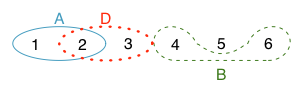
\includegraphics[scale=0.75]{images/sets.png}
    \end{center}
    Now we can see that $A$ and $B$ are disjoint; $D$ and $B$ are disjoint; but $A$ and $D$ are \textit{not} disjoint.
\end{frame}

\begin{frame}{Addition Rule for Sets?}
    The addition rule applies to sets in the same way that it applies to outcomes.
    
    \vspace{12pt}Keep $A=\{1,2\}$ and $B=\{4,6\}$. For our die, $P(A)=1/3$ and $P(B)=1/3$, so 
    \[
        P(A \text{ or } B)=P(A)+P(B)=(1/3)+(1/3)=2/3
    \]
\end{frame}

\begin{frame}{Probability for Non-Disjoint Events}
    We will use a standard 52 card deck to discuss disjoint events. If you are unfamiliar with the 52 card deck, it looks something like this:
    \begin{center}
        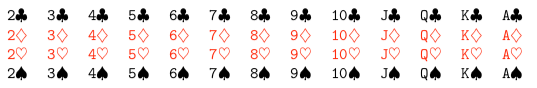
\includegraphics[scale=0.5]{images/cards.png}
    \end{center}
    \begin{itemize}
        \item 2 colors (\textcolor{red}{red} and black)
        \item 4 suits (clubs $\clubsuit$, spades $\spadesuit$, \textcolor{red}{diamonds} $\textcolor{red}{\diamondsuit}$, and \textcolor{red}{hearts} $\textcolor{red}{\heartsuit}$)
        \item In each suit, there are 13 cards labeled \texttt{2}, \texttt{3}, ..., \texttt{10}, \texttt{J} (jack), \texttt{Q} (queen), \texttt{K} (king), \texttt{A} (ace).
        \item The cards \texttt{J}, \texttt{Q}, and \texttt{K} are called the "face cards".
    \end{itemize}
\end{frame}

\begin{frame}{Venn Diagrams}
    A few slides ago, I suggested that drawing a picture might be helpful. A \textbf{Venn Diagram} is a good way to visualize the relationship between events.
    \begin{center}
        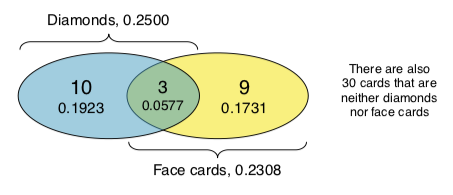
\includegraphics[scale=0.5]{images/venndiagram.png}
    \end{center}
    This Venn Diagram shows the events \texttt{Diamonds} and \texttt{Face Cards} as ovals. There are 3 face cards in the diamond suit, so the ovals overlap.
\end{frame}

\begin{frame}{Probability for Non-Disjoint Events}

    What if we want to know the probability that a randomly selected card is a \texttt{diamond} or a \texttt{face card}?

\end{frame}

\begin{frame}{Probability for Non-Disjoint Events}
    \begin{center}
        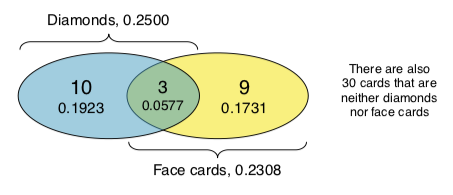
\includegraphics[scale=0.4]{images/venndiagram.png}
    \end{center}
    \begin{itemize}
        \item We start by adding up the probabilities
        \[
        P(\textcolor{red}{\diamondsuit})+P(\texttt{face card})=13/52 + 12/52
        \]
        \item But this double counts the 3 cards in the overlap!
    \end{itemize}
\end{frame}

\begin{frame}{Probability for Non-Disjoint Events}
    \begin{center}
        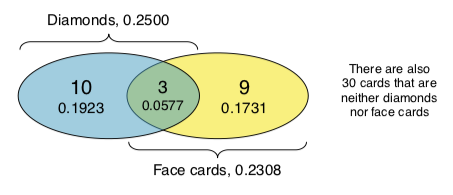
\includegraphics[scale=0.4]{images/venndiagram.png}
    \end{center}
    \begin{itemize}
        \item We need to correct for this double count:
        \begin{align*}
        P(\textcolor{red}{\diamondsuit} \text{ or } \texttt{face}) 
        & = P(\textcolor{red}{\diamondsuit})+P(\texttt{face}) - P(\textcolor{red}{\diamondsuit} \text{ and } \texttt{face}) \\
        & =13/52 + 12/52 -3/52 \\
        & = 22/52
        \end{align*}
    \end{itemize}
\end{frame}

\begin{frame}{Probability for Non-Disjoint Events}
    We can also confirm that this works by checking our deck.
    
    \begin{center}
        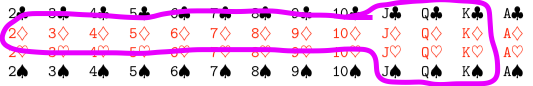
\includegraphics[scale=0.5]{images/cards2.png}
    \end{center}
    
    All of the cards that are a \texttt{diamond} or a \texttt{face card} are circled in purple. We can count that there are 22 of them. $22/52 = 0.42$ or 42\%.
\end{frame}

\begin{frame}{General Addition Rule}
    For any two events $A$ and $B$, the probability that at least one of them will occur is
    \[
        P(A \text{ or } B) = P(A) + P(B) - P(A \text{ and } B)
    \]
    where $P(A \text{ and } B)$ is the probability that both events occur.
    
    \vspace{18pt}Note: In statistics, whenever we say "or" we mean "and/or". If we say that "$A$ or $B$ occurs", that means $A$, $B$, or both $A$ and $B$ occur.
\end{frame}

\begin{frame}{General Addition Rule}
    By definition, for disjoint events $P(A \text{ and } B)=0$ (they can never occur simultaneously), so the general addition rule will work for both disjoint and non-disjoint events.
\end{frame}

\begin{frame}{Example}
    In the loans data set describing 10000 loans, 1495 loans were from joint applications, 4789 applicants had a mortgage, and 950 had both of these characteristics. Create a Venn diagram for this setup.
\end{frame}

\begin{frame}{Example}
    Using the Venn diagram, find the probability a randomly selected loan is from a joint application where the couple had a mortgage. What is the probability that the loan had either of these attributes (joint or mortgage)?
\end{frame}

\begin{frame}{Example}
    \textbf{Using the Venn diagram, find the probability a randomly selected loan is from a joint application where the couple had a mortgage.}
    
    \vspace{12pt}\[P(\text{joint and mortgage}) = 950/10000 = 0.095\]
\end{frame}

\begin{frame}{Example}
    \textbf{What is the probability that the loan had either of these attributes (joint or mortgage)?}
    
    \vspace{12pt}\begin{align*}
        P(\text{joint or mortgage}) &= P(\text{joint}) + P(\text{mortgage}) - P(\text{joint and mortgage}) \\
        &= (1495/10000)+(4789/10000)-(950/10000) \\
        &= 0.5334
    \end{align*}
\end{frame}

\begin{frame}{Probability Distributions}
    A \textbf{probability distribution} shows all possible (disjoint) outcomes and their corresponding probabilities.
    
    \vspace{12pt}\begin{center}
        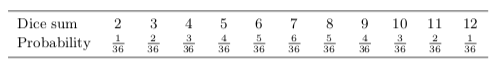
\includegraphics[scale=0.5]{images/sum2d6.png}
    \end{center}
    This is the probability distribution for the sum of two six-sided dice.
\end{frame}

\begin{frame}{Rules for Probability Distributions}
    A probability distribution is a list of the possible outcomes with corresponding probabilities that satisfies three rules:
    \begin{enumerate}
        \item The outcomes listed must be disjoint.
        \item Each probability must be between 0 and 1.
        \item The probabilities must sum to 1.
    \end{enumerate}
    
    \vspace{12pt}We can use these rules to check whether something is a valid probability distribution.
\end{frame}

\begin{frame}{Example: Rules for Probability Distributions}
    Let's start by checking our sums for the two six-sided dice.
    \vspace{12pt}\begin{center}
        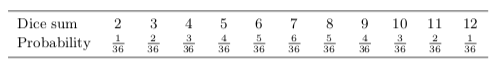
\includegraphics[scale=0.5]{images/sum2d6.png}
    \end{center}
    \begin{enumerate}
        \item The outcomes are disjoint (the two dice can't simultaneously sum to 3 \textit{and} 4).
        \item Each probability is between 0 and 1 (the minimum is 1/36 and the maximum is 6/36).
        \item The probabilities sum to 1
        \[
        \frac{1}{36}+\frac{2}{36}+\frac{3}{36}+\frac{4}{36}+\frac{5}{36}+\frac{6}{36}+\frac{5}{36}+\frac{4}{36}+\frac{3}{36}+\frac{2}{36}+\frac{1}{36}=\frac{36}{36}
        \]
    \end{enumerate}
\end{frame}

\begin{frame}{Example: Rules for Probability Distributions}
    The table below suggests 3 different distributions for household income in the US. Which one is a valid probability distribution? Why?
    
    \vspace{12pt}\begin{tabular}{r|cccc}
        \hline
        Income Range & \$0-25k & \$25k-50k & \$50k-100k & \$100k+ \\ \hline
        (a) & 0.18 & 0.39 & 0.33 & 0.16 \\
        (b) & 0.38 & -0.27 & 0.52 & 0.37 \\
        (c) & 0.28 & 0.27 & 0.29 & 0.16\\ \hline
    \end{tabular}
\end{frame}

\begin{frame}{Example: Rules for Probability Distributions}
    \begin{tabular}{r|cccc}
        \hline
        Income Range & \$0-25k & \$25k-50k & \$50k-100k & \$100k+ \\ \hline
        (a) & 0.18 & 0.39 & 0.33 & 0.16 \\
        (b) & 0.38 & -0.27 & 0.52 & 0.37 \\
        (c) & 0.28 & 0.27 & 0.29 & 0.16\\ \hline
    \end{tabular}
    
    \vspace{12pt}Let's check (a):
    \begin{enumerate}
        \item The outcomes listed must be disjoint. (TRUE)
        \item Each probability must be between 0 and 1. (TRUE)
        \item \textbf{The probabilities must sum to 1.}
        \begin{itemize}
            \item $0.18+0.39+0.33+0.16=1.16$
        \end{itemize}
    \end{enumerate}
\end{frame}

\begin{frame}{Example: Rules for Probability Distributions}
    \begin{tabular}{r|cccc}
        \hline
        Income Range & \$0-25k & \$25k-50k & \$50k-100k & \$100k+ \\ \hline
        (a) & 0.18 & 0.39 & 0.33 & 0.16 \\
        (b) & 0.38 & -0.27 & 0.52 & 0.37 \\
        (c) & 0.28 & 0.27 & 0.29 & 0.16\\ \hline
    \end{tabular}
    
    \vspace{12pt}Checking (b),
    \begin{enumerate}
        \item The outcomes listed must be disjoint. (TRUE)
        \item \textbf{Each probability must be between 0 and 1.}
        \begin{itemize}
            \item $P(\text{\$25k-50k})=-0.27$
        \end{itemize}
        \item The probabilities must sum to 1. (TRUE)
    \end{enumerate}
\end{frame}

\begin{frame}{Example: Rules for Probability Distributions}
    \begin{tabular}{r|cccc}
        \hline
        Income Range & \$0-25k & \$25k-50k & \$50k-100k & \$100k+ \\ \hline
        (a) & 0.18 & 0.39 & 0.33 & 0.16 \\
        (b) & 0.38 & -0.27 & 0.52 & 0.37 \\
        (c) & 0.28 & 0.27 & 0.29 & 0.16\\ \hline
    \end{tabular}
    
    \vspace{12pt}And checking (c),
    \begin{enumerate}
        \item The outcomes listed must be disjoint. (TRUE)
        \item Each probability must be between 0 and 1. (TRUE)
        \item The probabilities must sum to 1. (TRUE)
    \end{enumerate}
    So (c) is our valid probability distribution.
\end{frame}

\begin{frame}{Visualizing Probability Distributions}
    We can visualize this probability distribution using a bar plot.
    \begin{center}
        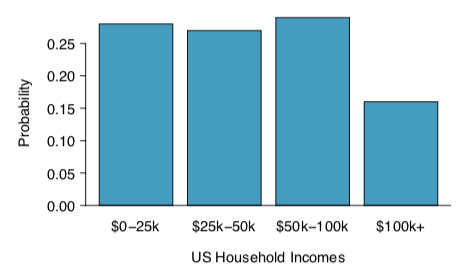
\includegraphics[scale=0.5]{images/probplot.png}
    \end{center}
    This is very similar to what we did when we created bar plots for proportion-based summary tables.
\end{frame}

\begin{frame}{Visualizing Probability Distributions}
    \begin{center}
        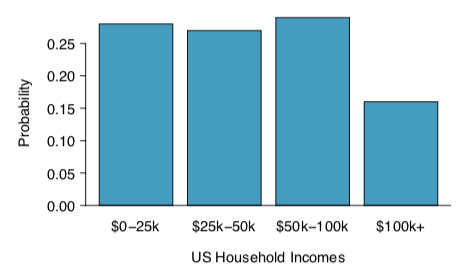
\includegraphics[scale=0.4]{images/probplot.png}
    \end{center}
    In these bar plots, the heights of the bars represent the probabilities of each event.
\end{frame}

\begin{frame}{Visualizing Probability Distributions}
    \begin{center}
        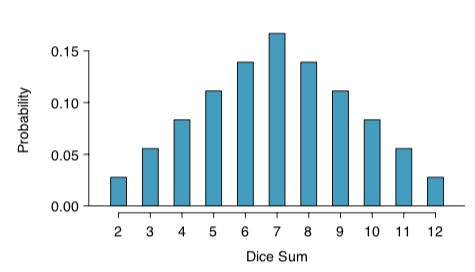
\includegraphics[scale=0.5]{images/dicesumplot.png}
    \end{center}
    This plot shows the probability distribution for the sum of the two six-sided dice.
\end{frame}

\begin{frame}{Sample Space}
    \begin{itemize}
        \item Rolling our six-sided die results in some event in the set $S=\{1,2,3,4,5,6\}$.
        \item We call this set our \textbf{sample space} ($S$). 
        \item The sample space is defined as the set of all possible outcomes.
    \end{itemize}
\end{frame}

\begin{frame}{Complement of an Event}
    Let $D=\{2,3\}$ be the event that a single roll of our d6 is a \texttt{2} or a \texttt{3}. 
    \begin{itemize}
        \item The \textbf{complement} of $D$ is the set of events in the sample space that are \textit{not} in $D$.
        \item We denote the complement by $D^c$.
        \item Then $D^c = \{1,4,5,6\}$
    \end{itemize}
    \begin{center}
        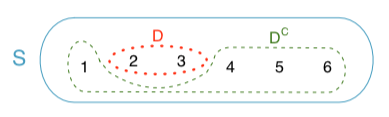
\includegraphics[scale=0.5]{images/comp.png}
    \end{center}
\end{frame}

\begin{frame}{Example: Complement of an Event}
    Let $D=\{2,3\}$ be the event that a single roll of our d6 is a \texttt{2} or a \texttt{3}. 
    
    \vspace{12pt}Find $P(D \text{ or } D^c)$. 
\end{frame}

\begin{frame}{Example: Complement of an Event}
    Let $D=\{2,3\}$ be the event that a single roll of our d6 is a \texttt{2} or a \texttt{3}. 
    
    \vspace{12pt}Find $P(D \text{ or } D^c)$. 
    \begin{itemize}
        \item First, note that an event and it's complement are always disjoint!
        \item So 
        \begin{align*}
            P(D \text{ or } D^c) &= P(D)+P(D^c) \\
            &= (1/3) + (2/3) \\
            &= 1
        \end{align*}
    \end{itemize}
\end{frame}

\begin{frame}{Example: Complement of an Event}
    Think back to possible rolls for our six-sided die. Let $A=\{1,2\}$, the event that we roll a \texttt{1} or a \texttt{2}, and $B=\{4,6\}$, the event of a \texttt{4} or a \texttt{6}.
    \begin{enumerate}
        \item What do $A^c$ and $B^c$ represent?
        \item Compute $P(A^c)$ and $P(B^c)$.
        \item Compute $P(A)+P(A^c)$ and $P(B)+P(B^c)$.
    \end{enumerate}
\end{frame}

\begin{frame}{Properties of the Complement}
    \begin{itemize}
        \item Every possible outcome not in $A$ is in $A^c$, so ($A$ or $A^c$) encompasses the entire sample space.
        \item So $P(A \text{ or } A^c)$ is the same as $P(S)$
        \item $P(S)=1$, always! 
        \begin{itemize}
            \item $S$ is all possible outcomes and there is a 100\% chance that we observe at least one of the possible outcomes.
        \end{itemize}
    \end{itemize}
\end{frame}

\begin{frame}{Properties of the Complement}
    So we can write
    \[
    P(A \text{ or } A^c) = P(A)+P(A^c)=1
    \]
    and 
    \[
    P(A) = 1-P(A^c)
    \]
    
    \vspace{12pt}Using this relationship with the complement can help us deal with more complex probability problems down the line.
\end{frame}

\begin{frame}{Example}
    \begin{center}
        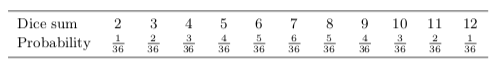
\includegraphics[scale=0.5]{images/sum2d6.png}
    \end{center}
    Use the probability distribution to compute the following probabilities for rolling two six-sided dice:
    \begin{enumerate}
        \item The sum of the dice is not 6.
        \item The sum is at least 4. That is, determine the probability of the event $B = \{4, 5, ..., 12\}$.
        \item The sum is no more than 10. That is, determine the probability of the event $D = \{2, 3, ..., 10\}$.
    \end{enumerate}
\end{frame}

\begin{frame}{Example: Find $P$(sum not 6).}
    We could add all of the probabilities for the sums that are not 6... or we could use the complement!
    \begin{itemize}
        \item Let $A=\{\text{not 6}\}$ be the event that the sum is not 6.
        \item Then $A^c=\{6\}$, the event that the sum is 6.
        \item Recall 
        \begin{align*}
            P(A) &=1-P(A^c) \\
            & =1-P(6) \\
            & =1-\frac{5}{36} \\
            &= 31/36
        \end{align*}
    \end{itemize}
\end{frame}

\begin{frame}{Example: Find $P$(sum at least 4).}
    Now, we want to know if the sum is \textit{at least} 4. This means that we want to know if the sum is greater than \textit{or equal to} 4.
    \begin{itemize}
        \item Let $B=\{4,5,\dots,12\}$ be the event that the sum is at least 4.
        \item Then $B^c=\{2,3\}$, the event that the sum is less than 4.
    \end{itemize}
    \begin{align*}
            P(B) &=1-P(B^c) \\
            & =1-P(\{2,3\}) \\
            & =1-[P(3)+P(2)] \\
            & =1-\left[\frac{2}{36}+\frac{1}{36}\right] \\
            & =1-(3/36) \\
            & =11/12
        \end{align*}
\end{frame}

\begin{frame}{Example: Find $P$(sum no more than 10).}
    Now, we want to know if the sum is \textit{no more than} 10. This means that we want to know if the sum is less than \textit{or equal to} 10.
    \begin{itemize}
        \item Let $D=\{2,3,\dots,10\}$ be the event that the sum is no more than 10.
        \item Then $D^c=\{11,12\}$, the event that the sum is greater than 10.
    \end{itemize}
    \begin{align*}
            P(D) &=1-P(D^c) \\
            & =1-P(\{11,12\}) \\
            & =1-[P(11)+P(12)] \\
            & =1-\left[\frac{2}{36}+\frac{1}{36}\right] \\
            & =1-(3/36) \\
            & =11/12
        \end{align*}
\end{frame}

\begin{frame}{Midterm}
    The Midterm is next week Tuesday, August 13.
    \begin{itemize}
        \item Approximately 50 multiple choice questions.
        \item You do not need a scantron.
        \item Questions will be mostly conceptual.
        \item You may bring any basic or graphing calculator.
        \item I will bring extra scratch paper.
    \end{itemize}
\end{frame}

\begin{frame}{Extra Credit Opportunity}
    \begin{itemize}
        \item Write an exam question that would be appropriate for your midterm. 
        \item The midterm will cover material from Chapters 1, 2, and 3. 
        \item Your exam question must come from material covered in class, your homeworks, or your labs. 
        \item Questions may be either multiple choice or short answer. 
        \item To receive any credit, you must write an original question and provide both the question and the correct answer.
    \end{itemize}
    These can be submitted on iLearn (Assignments tab). It opens today at 9:30am and will close on Thursday at 11:59pm.
\end{frame}

\begin{frame}{Independence}
    \begin{itemize}
        \item Independence of random processes is similar to independence of variables and observations.
        \item We say that two random processes are \textbf{independent} if knowing the outcome of one provides no useful information about the outcome of the other.
    \end{itemize}
\end{frame}

\begin{frame}{Independence}
    For example, consider our discussion on rolling 2 six-sided dice.
    \begin{itemize}
        \item The roll of the first die has no effect on the roll of the second die.
        \item Thus our two dice rolls are independent of one another. 
    \end{itemize}
\end{frame}

\begin{frame}{Independence}
    We've already calculated the probability of the two rolls both being a \texttt{1}
    \begin{itemize}
        \item 1/6 of the time the first roll is a \texttt{1}
        \item A further 1/6 of \textit{those} times the second is also a \texttt{1}.
        \item So we decided that the probability was $(1/6)\times(1/6)=1/36$.
    \end{itemize}
    Multiplying these probabilities together works because the two events are independent.
\end{frame}

\begin{frame}{Multiplication Rule for Independent Processes}
    Let $A$ and $B$ be events from two different and independent processes. Then the probability that both $A$ and $B$ occur can be calculated as the product of their separate probabilities:
    \[ 
        P (A\text{ and }B) = P (A) \times P (B)
    \]
    Similarly, if there are $k$ events $A_1, \dots, A_k$ from $k$ independent processes, then the probability they all occur is
    \[
        P(A_1)\times P(A_2)\times\dots\times P(A_k)
    \]
\end{frame}

\begin{frame}{Example}
    About 9\% of people are left-handed. Suppose 2 people are selected at random from the U.S. population. Because the sample size of 2 is very small relative to the population, it is reasonable to assume these two people are independent.
    \begin{enumerate}
        \item What is the probability that both are left-handed?
        \item What is the probability that both are right-handed?
    \end{enumerate} 
\end{frame}

\begin{frame}{Example: Both Left-Handed}
    \textbf{What is the probability that both are left-handed?}
    \begin{itemize}
        \item Let $L_1$ be the event that the first person is left-handed and $L_2$ the event that the second person is left-handed.
        \item We are told that 9\% of people are left-handed, so $P(L_1)=P(L_2)=0.09$.
    \end{itemize}
\end{frame}

\begin{frame}{Example: Both Left-Handed}
    \textbf{What is the probability that both are left-handed?}
    \begin{itemize}
        \item We are assuming that these people are independent, so we can use the multiplication rule:
        \begin{align*}
        P(L_1\text{ and }L_2) &= P(L_1) \times P(L_2) \\
        &= (0.09)\times(0.09) \\
        &= 0.0081
        \end{align*}
        or 0.81\% (this is highly unlikely!)
    \end{itemize}
\end{frame}

\begin{frame}{Example: Both Right-Handed}
    \textbf{What is the probability that both are right-handed?}
    \begin{itemize}
        \item First, assume that everyone is either right- or left-handed.
        \item Then $L_1^c$ is the event that the first person is right-handed and $L_2^c$ is the event that the second person is right-handed.
        \item From the previous slide, we decided that $P(L_1)=P(L_2)=0.09$
        \item So $P(L_1^c)=1-P(L_1)=1-0.09=0.91$ and $P(L_2^c)=0.91$
    \end{itemize}
\end{frame}

\begin{frame}{Example: Both Right-Handed}
    \textbf{What is the probability that both are right-handed?}
    \begin{itemize}
        \item We are still assuming that these people are independent, so we can again use the multiplication rule:
        \begin{align*}
        P(L_1^c\text{ and }L_2^c) &= P(L_1^c) \times P(L_2^c) \\
        &= (0.91)\times(0.91) \\
        &= 0.8281
        \end{align*}
        or 82.81\%.
    \end{itemize}
\end{frame}

\begin{frame}{Disjoint Events - Independent?}
    If two events are disjoint, are they independent?
\end{frame}

\begin{frame}{Disjoint Events- Independent?}
    If two events are disjoint, are they independent?
    \begin{itemize}
        \item Recall that independent events have no relationship with one another.
        \item This means that if we know something about event $A$, we don't get any information about event $B$.
        \item For disjoint events, if event $A$ occurs, we can be totally certain that event $B$ did not occur.
        \item Therefore they are \textit{dependent}.
    \end{itemize}
\end{frame}

\begin{frame}{Example}
    Consider two disjoint events for rolling a six-sided die. Let $A=\{1\}$ be the event that I roll a \texttt{1} and $B=\{2\}$ the event that I roll a \texttt{2}. 
    \begin{itemize}
        \item If I know that $A$ occurred, then I can be 100\% sure that $B$ did not occur.
        \item If I know that $A$ did not occur, then I know that the roll must be a \texttt{2}, \texttt{3}, \texttt{4}, \texttt{5}, or \texttt{6}. 
        \begin{itemize}
            \item Now there are five possible options instead of six!
            \item We've narrowed down our options, so knowing that I did not roll a \texttt{1} has given us some useful information.
        \end{itemize}
    \end{itemize}
    Therefore $A$ and $B$ can't be independent.
\end{frame}